\subsection{Connection patterns for hardware design and parallel programming}\label{sec:combinators}

Connection patterns that capture common ways to connect sub-circuits into larger structures have been central to our research on functional and relational languages for hardware design.
Inspired by Backus' FP language, Sheeran's early work on $\mu$FP made use of
{\em combining forms} with geometric interpretations~\citeifl{SheeranLFP84}. This approach
to capturing circuit regularity was also influenced by contact
with designers of regular array circuits in industry -- see reference~\citeifl{SheeranJUCS} for an overview of this and much other work on functional programming and hardware design.

Later work on (our) Ruby considered the use of binary relations, rather than functions in specifying hardware~\citeifl{LyngbyRuby}. Lava builds upon these ideas, but also gains much in expressiveness and flexibility by being embedded in Haskell~\citeifl{lavaICFP,ClaessenThesis}.
The user writes what look like circuit descriptions, but are in fact circuit {\em generators}. Commonly used {\em connection patterns} are captured by higher order functions.

For example, an important pattern is parallel prefix or scan. Given inputs\newline $[x_0, x_1 \ldots x_{n-1}]$, the prefix problem is to compute each $x_0 \circ x_1 \circ \ldots \circ x_j$ for $0 \leq j < n$, for $\circ$ an associative, but not necessarily commutative, operator. For example, the prefix sum of {\tt [1..10]} is {\tt [1,3,6,10,15,21,28,36,45,55]}. There is an obvious sequential solution, but in circuit design one is often aiming for a circuit that exploits parallelism, and so is faster (but also larger). In a construction attributed to Sklansky, one can perform the prefix
calculation by first, recursively, performing the prefix calculation on 
each half of the input, and then combining (via the operator) the last output of the first of these
recursive calls with each of the outputs of the second.
For instance, to calculate the prefix sum of {\tt [1..10]}, one can compute the prefix
sums of {\tt [1..5]} and {\tt [6..10]}, giving {\tt [1,3,6,10,15]}
and {\tt [6,13,21,30,40]}, respectively. 
The final step is to add the last element of the output of the first recursive call ({\tt 15}) to each element of
the output of the second.

To express the construction in Lava, we make use of two connection patterns.\newline
{\tt two :: ([a] -> [b]) -> [a] -> [b]} applies its component to
the top and bottom halves of the input list, concatenating the two sub-lists
that result from these applications.
Thus, {\tt two (sklansky plus)} applied to {\tt [1..10]} gives {\tt [1,3,6,} {\tt10,15,6,13,21,30,40]}.
Left-to-right serial composition has type
{\tt (a -> b) -> (b -> c) -> a -> c} and is written as infix {\tt ->-}.
The description of the construction mixes the use of connection patterns, giving a form of reuse, with the naming of ``wires''.

\begin{code}
sklansky :: ((t, t) -> t) -> [t] -> [t]
sklansky op [a] = [a]
sklansky op as = (two (sklansky op) ->- sfan) as
  where
    sfan as = a1s ++ a2s'
      where
        (a1s,a2s) = splitAt ((length as + 1) `div` 2) as
        a2s'      = [op(last a1s,a) | a <- a2s]

*Main> simulate (sklansky plus) [1..10]
[1,3,6,10,15,21,28,36,45,55]
\end{code}

Lava supports simulation, formal verification and netlist generation from definitions like this. Circuit descriptions are {\em run} (in fact symbolically evaluated) in order to produce an intermediate representation, which is in turn written out in various formats (for fixed size instances). So this is an example of {\em staged programming}~\citeifl{Taha03}.

The Sklansky construction is one way to implement parallel prefix, and there are many others, see for instance Hinze's excellent survey~\citeifl{Hinze}.
Those who develop prefix algorithms suitable for hardware implementation use a standard notation to represent
the resulting networks. Data flows from top to bottom and
the least significant input is at top left. Black dots represent
operators.
For example, Figure~\ref{fig:skl32} shows the
recursive Sklansky construction for 32 inputs. 
%
\begin{figure}%
\begin{center}
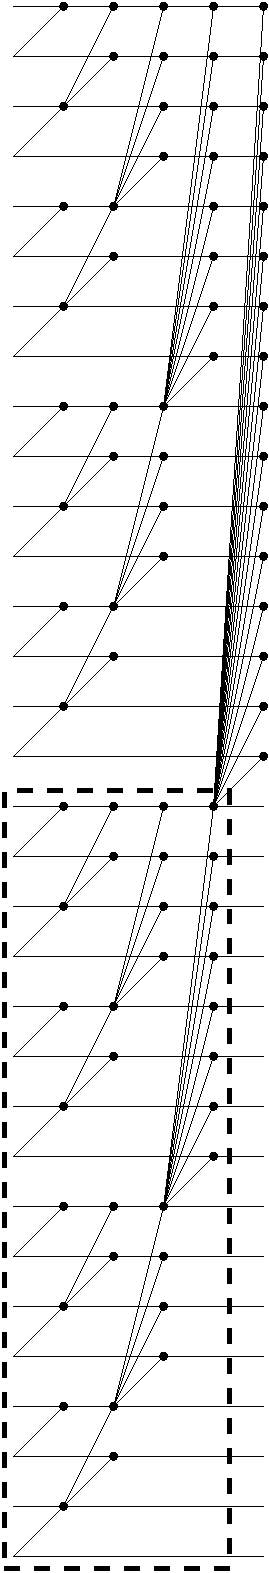
\includegraphics[bb=0 0 123 748, angle=270, scale=0.4]{./ifl/skl32.pdf}
\caption{The Sklansky construction for $32$ inputs. 
It recursively computes the parallel prefix for each half of the inputs (corresponding to the use of {\tt two} in the definition) and then combines the last output of the lower (left) half with each of the outputs of the upper (right) half. The dotted box outlines the recursive call on the lower half of the inputs.}\label{fig:skl32}
\end{center}
\end{figure}

In this work, we plan to investigate the use of connection patterns, and more generally an emphasis on {\em structure}, in parallel programming.
We have chosen to target GPUs partly because of available expertise among our colleagues at Chalmers, and partly because reading papers about General Purpose GPU (GPGPU) programming gave us a sense of d{\'e}j\`a vu. Programs are illustrated graphically, and bear a remarkable resemblance to circuit modules that we have
generated in the past using Lava. We see an opportunity here, as there is an extensive literature, going back to the 1960s, about implementing algorithms on silicon that may provide clues
about implementing algorithms on GPUs. This literature does not seem to have yet been scrutinised by the Data Parallel Programming or GPGPU communities.
This is possibly because GPUs are moving closer to simply being data parallel machines, and so work on library functions has taken inspiration from earlier work on Data Parallel Programming, such as Blelloch's NESL~\citeifl{NESL}. But some of the restrictions from the early data parallel machines no longer hold today; for instance broadcasting a value to many processors was expensive in the past, but is much easier to do on modern GPUs. So a construction like Sklansky, which requires such broadcasting, should now be reconsidered, and indeed we have found it to give good results in our initial experiments (writing directly in CUDA). In general, it makes sense to spread the net beyond the standard data parallel programming literature when looking for inspiration in parallel algorithm design. We plan to explore the use of ``old'' circuit design ideas in programming library functions for GPUs.

Below, we briefly review modern GPUs and a standard programming model.




